\section{File usability and data access patterns}
One of the key parameters to assess our effective storage usage is to measure the access frequency after data placement. The two extremes regarding data thermodynamics are \emph{cold data} where files are WORN (Write Once Read Never) and \emph{hot data} where files are accessed quickly after data placement and with high concurrency. After studying data access patterns at several sites we observed that large fraction of our files are neither totally \emph{cold} nor \emph{hot}. The analysis files lose popularity with time and the access rate decreases significantly after days/weeks, in (Fig. \ref{access}) the file rates and file popularity on a Tier-1 and a Tier-2 are shown as a function of time as a representative example.

\begin{figure}[h]
  \centering
  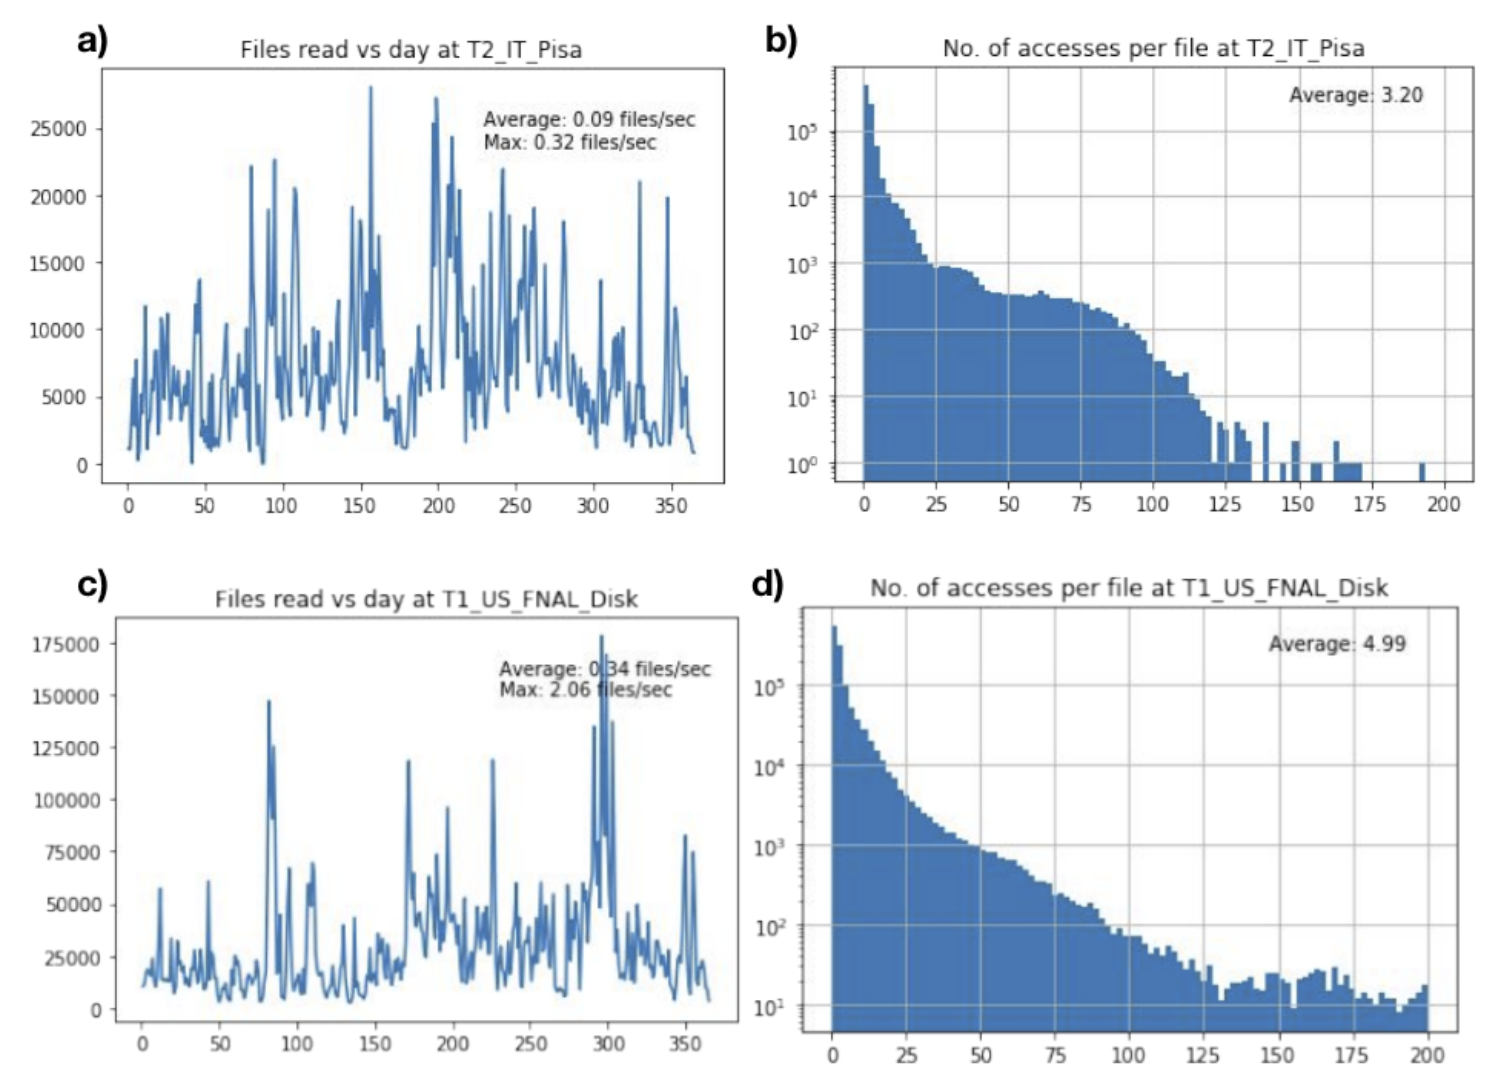
\includegraphics[height=8cm]{dataaccess-chep2019.png}
  \caption{{\em (left)} File popularity on a Tier-1 and a Tier-2 as a function of time (300 days). The plots above indicate that data is not accessed very often, it is most likely to be re-read within days after placement then the access drops substantially, almost two orders of magnitude.}
  \label{access}
\end{figure}

This provides an indication whether this type of data could be better accessed through a cache, so it is available when is popular and gets super-seeded with newer files once they are less demanded. In this way the space on disk at the computing sites is optimised for data being actively used and this can potentially be completely delegated to an \emph{stateless} cache. In parallel less frequently used data might be re-fetched again from the Data Lake (disk or tape) where the experiments will handle the popularity with the required Quality of Service (QoS) to make use of the best cost/usage ratio for the storage.\\
We also observed a fundamental difference between analysis and production data. Analysis has higher re-use while production files have very few re-reads. As a result running combined workflows on a site has the effect to push analysis data out of the cache.

%This made us think that in the case we do not change much of the current infrastructure we would nevertheless benefit by changing the current model and favoring running predictable and time-defined workflows at the sites with less storage and favor less-predictable user analysis on sites with larger storage services.\\

It should be noted that these observations are based only on a period of six months but they provide hints towards a cache-oriented storage. Further studies should be done on longer period and also combined with staging and data deletion information. 
